\documentclass{article}
\usepackage[english]{babel}
\usepackage{longtable}
\usepackage[top=1in, bottom=0.25in, left=1.25in, right=1.25in,includefoot,heightrounded]{geometry}
\usepackage{indentfirst}
\usepackage[utf8]{inputenc}
\usepackage{amsmath,amssymb}
\usepackage{graphicx,tikz}
\usepackage{hyperref}
\usepackage[colorinlistoftodos]{todonotes}
\usepackage[document]{ragged2e}
\usepackage{fancyhdr}
\usepackage{enumerate}
\usepackage{listings}
\usepackage{color}
\usepackage{flowchart}
\usepackage{hyperref}
\usepackage{graphicx}
\usetikzlibrary{arrows}


\usetikzlibrary{shapes.geometric, arrows}
\tikzstyle{startstop} = [rectangle, rounded corners, minimum width=3cm, minimum height=1cm,text centered, draw=black, fill=red!30]
\tikzstyle{decision} = [diamond, minimum width=4cm, minimum height=0.5cm, text centered, draw=black, fill=green!30]
\tikzstyle{process} = [rectangle, minimum width=3cm, minimum height=1cm, text centered, draw=black, fill=orange!30]
\tikzstyle{arrow} = [thick,->,>=stealth]
\tikzstyle{io} = [trapezium, trapezium left angle=70, trapezium right angle=110, minimum width=2cm, text width=4cm, minimum height=1cm, text centered, draw=black, fill=blue!30]

\pagestyle{fancy}
\fancyhf{}
\lhead{Myles Deslippe}
\rhead{Comp 3670 | Computer Networks}
\cfoot{\thepage}

\definecolor{MyDarkGreen}{rgb}{0.0,0.4,0.0}
\lstset{inputencoding=ansinew}
\lstset{breaklines=true} 

\begin{document}

    \section*{\centering{Introduction}}

    \subsection*{Network Hosts and Communication Links}
    \begin{itemize}
        \item A \textbf{network host} is a computational device that is connected to a network.
        \item \textbf{Hosts} may work as a \textbf{server} offering \textbf{information resources, services, and applications} to users and other hosts.
        \item \textbf{Hosts} are assigned a unique \textbf{network address}.
        \item The \textbf{network edge} refers to the area where a \textbf{device or local network interfaces with a large network}.
        \item A \textbf{link} is a \textbf{communication channel} that connects two or more devices for the purpose of \textbf{data transmission}.
        \item \textbf{Bandwidth} refers to the \textbf{maximum rate data can be transmitted over a link}.
    \end{itemize}
    
    \subsection*{Packets and Packet Switching}
    \begin{itemize}
        \item \textbf{Packet Switching} is a method of \textbf{grouping data into packets} that are transmitted over a network.
        \item A \textbf{network packet} is a formatted unit of data carried by a \textbf{packet-switched network}.
        \item \textbf{Packets} consist of \textbf{control information, and the payload}.
    \end{itemize}

    \subsection*{Network Devices}
    \begin{itemize}
        \item A \textbf{modem} or a \textbf{modulator-demodulator} is a computer networking device that \textbf{converts data} between a \textbf{digital format, and an analog format} for the purpose of transmission.
        \item A \textbf{router} is a computer networking device that \textbf{creates and manages a local network}, and \textbf{manages the data entering and exiting the network}.
        \item A \textbf{switch} is a computer networking device that \textbf{connects devices via packet switching} to \textbf{receive and forward data}.
        \item \textbf{Routers use IP addresses} to route data, and \textbf{switches use MAC addresses} to route data.
    \end{itemize}

    \subsection*{Network Terminologies}
    \begin{itemize}
        \item A \textbf{bit (binary digit)} is a single unit of information.
        \item A \textbf{physical link} is the physical \textbf{communication link} that \textbf{connects transmitters and receivers}.
        \item \textbf{Guided media} refers to signals that \textbf{propagate in a solid medium}.
        \item \textbf{Unguided media} refers to \textbf{signals that propagate freely}. 
        \item \textbf{Routing} refers to the process of determining the \textbf{path a packet will take} to reach it's destination.
        \item \textbf{Forwarding} refers to the \textbf{process of receiving a packed, and sending it to the next node in the path}. 
    \end{itemize}

\section*{\centering{The Internet}}

    \subsection*{The Internet}
    \begin{itemize}
        \item \textbf{The Internet} is a \textbf{global computer network} that provides a variety of \textbf{information and communication facilities}.
        \item \textbf{The Internet} consists of \textbf{interconnected networks} using \textbf{standardized communication protocols}.
        \item A \textbf{communication protocol} is a \textbf{system of rules that allows two or more entities to communicate of the internet}.
        \item \textbf{Protocols} define the \textbf{rules, syntax, semantics, and synchronization} of the communication.
        \item The \textbf{internet network core} refers to the infrastructure (routers) that connect networks together.
   \end{itemize}

   \subsection*{Internet Service Providers and Access Networks}
   \begin{itemize}
       \item An \textbf{Internet service provider} is an organization that \textbf{provides services for accessing, and using the internet}.
       \item One way an \textbf{ISP} can provide their customers with \textbf{internet access} is through \textbf{existing telephone lines (Digital Subscriber Lines or DLS)}.
       \item \textbf{DSL} was mainly used when the \textbf{internet was first created}, and is often referred to as \textbf{dial up}.
       \item The \textbf{problem} with \textbf{DLS} is that it only supports a single connection.
       \item A more-modern way \textbf{ISPs} provide their customers with \textbf{internet access} is with \textbf{cable-based access}.
       \item \textbf{Cable-based access} uses \textbf{frequency division multiplexing (FDM)} to \textbf{transmit data in different channels} allowing for several connections simultaneously.
       \item There are different types of \textbf{cables} such as \textbf{Hybrid Fiber Coax (HFC)}, and \textbf{Fiber Optic Cables}.
       \item Another way \textbf{ISPs} provide their customers with \textbf{internet access} is through \textbf{wireless access points (WAPs)}.
       \item \textbf{WAPs use electromagnetic radiation} to \textbf{transmit information} over different frequencies.
   \end{itemize}

   \subsection*{The Network Core}
   \begin{itemize}
       \item \textbf{The Network Core} is a mesh of \textbf{interconnected routers} that use \textbf{packet-switching} to transmit data.
       \item \textbf{Transmission delay} refers to the amount of time it takes for a packet to transmit.
       \item \textbf{Transmission delay} can be \textbf{calculated} with the following formula $\text{Delay}=\frac{L}{R}$ where $L$ is the \textbf{length of the packet}, and $R$ is the \textbf{transmission rate of the link in bits per second}.
       \item \textbf{Routers} use the \textbf{store and forward principal}; before they can \textbf{forward packets}, they have to \textbf{wait until the entire packet has arrived}.
       \item If the \textbf{arrival rate} of a packet \textbf{exceeds the transmission rate of a link} the packet will be \textbf{placed into a queue} for a short period of time; If the queue \textbf{runs out of memory} unsent packets will be \textbf{overwritten, causing packet loss}.
   \end{itemize}

   \subsection*{The Internet Structure}
   \begin{itemize}
       \item \textbf{Hosts} connect to the internet via \textbf{Access Internet Service Providers}.
       \item \textbf{ISPs are then interconnected}.
       \item There are different \textbf{tiers} of ISPs:
       \item[] 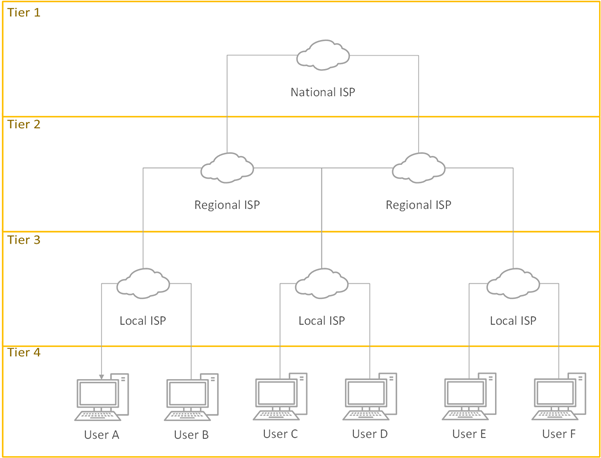
\includegraphics[height=175px]{images/ISP-Structure.png}
       \item The \textbf{ISP tiers} can have \textbf{peer-to-peer links} where they are \textbf{directly connected}, or they can have an \textbf{internet exchange point} which is an external network where \textbf{several networks can exchange data}.
       \item \textbf{Context network providers} (Google, Microsoft, etc) may also run \textbf{their own networks} that are connected to the \textbf{internet}.
   \end{itemize}

   \subsection*{Packet Delay}
   \begin{itemize}
       \item \textbf{Packet delay} refers to the \textbf{amount of time} it takes for a packet to \textbf{reach it's destination}.
       \item There are \textbf{four sources of packet delay} at a given \textbf{router}:
       \begin{enumerate}
           \item \textbf{Processing delay} - The amount of time it takes the \textbf{router to process the packet}.
           \item \textbf{Queuing delay} - The amount of time the \textbf{packet is queued for}.
           \item \textbf{Transmission delay} - The amount of time the \textbf{router takes to transmit the packet}.
           \item \textbf{Propagation delay} - The amount of time it takes the \textbf{link to transfer the packet}.
       \end{enumerate}
   \end{itemize}

   \subsection*{Network Throughput}
   \begin{itemize}
       \item \textbf{Network Throughput} refers to the \textbf{rate of successful message deliveries} over a communication channel.
       \item \textbf{Network Throughput} is measured in \textbf{bits / time unit}.
   \end{itemize}

   \subsection*{Protocol Layers}
   \begin{itemize}
       \item Most \textbf{network protocols} are structured as a \textbf{series of layers}, collectively referred to as a \textbf{protocol stack}.
       \item Each layer in a \textbf{protocol stack} is designed for a \textbf{specific purpose}.
   \end{itemize}

   \subsection*{The Internet Protocol Stack}
   \begin{itemize}
       \item \textbf{The internet} uses the \textbf{Transmission Control Protocol / Internet Protocol (TCP/IP) stack}.
       \item \textbf{TCP/IP} is composed of \textbf{5 layers}:
       \begin{enumerate}
           \item The \textbf{Physical Layer (Layer 1)} is the layer responsible for \textbf{moving data within a link}.
           \item The \textbf{Data-Link Layer (Layer 2)} is the layer responsible for \textbf{moving data in and out of the link}.
           \item The \textbf{Network Layer (Layer 3)} \textbf{controls the flow and routing traffic} to ensure data is sent efficiently and accurately.
           \item The \textbf{Transport Layer (Layer 4)} provides a \textbf{reliable data connection} over a network.
           \item The \textbf{Application Layer (Layer 5)} is the group of applications that \textbf{let the user access the network}.
       \end{enumerate}
   \end{itemize}

   \subsection*{TCP/IP Message Units}
   \begin{itemize}
       \item At \textbf{each layer} the unit of data has a different name.
       \item At \textbf{Layer 1 (Physical)} each unit of data is called a \textbf{bit}.
       \item At \textbf{Layer 2 (Data-Link)} each unit of data is called a \textbf{frame}.
       \item At \textbf{Layer 3 (Network)} each unit of data is called a \textbf{packet}.
       \item At \textbf{Layer 4 (Transport)} each unit of data is called a \textbf{segment}.
       \item At \textbf{Layer 5 (Application)} each unit of data is called a \textbf{message}.
   \end{itemize}

   \subsection*{The Open Systems Interconnection Model (OSI Model)}
   \begin{itemize}
       \item The \textbf{OSI model} is a \textbf{reference model} for how \textbf{applications communicate over a network}.
       \item The \textbf{OSI model} focuses on providing a \textbf{visual design} of how each \textbf{communication layer} is build \textbf{on top of the other}.
       \item The \textbf{OSI model} is composed of \textbf{7 layers}:
       \begin{enumerate}
        \item The \textbf{Physical Layer (Layer 1)} is the layer responsible for \textbf{moving data within a link}.
        \item The \textbf{Data-Link Layer (Layer 2)} is the layer responsible for \textbf{moving data in and out of the link}.
        \item The \textbf{Network Layer (Layer 3)} \textbf{controls the flow and routing traffic} to ensure data is sent efficiently and accurately.
        \item The \textbf{Transport Layer (Layer 4)} provides a \textbf{reliable data connection} over a network.
        \item The \textbf{Session Layer (Layer 5)} \textbf{manages the conversations that occur between applications}.
        \item The \textbf{Presentation Layer (Layer 6)} \textbf{translates or formats data} for the \textbf{application layer}. This layer also handles \textbf{encrypting and decrypting} the data the application layer requires.
        \item The \textbf{Application Layer (Layer 7)} is the group of applications that \textbf{let the user access the network}.
    \end{enumerate}
   \end{itemize}

    \section*{\centering{Network Security}}

    \subsection*{Network Security}
    \begin{itemize}
        \item \textbf{Network Security} is a set of technologies that \textbf{protects} the \textbf{usability, and integrity of network infrastructure}.
        \item A \textbf{network security architecture} is composed of \textbf{tools that protect the network itself and the applications that rely on it}.
    \end{itemize}

    \subsection*{Types of Dangers on a Network}
    \begin{itemize}
        \item \textbf{Malware (malicious software)} refers to \textbf{software} created by people with \textbf{bad intentions} that performs \textbf{malicious actions on the device / network}.
        \begin{itemize}
            \item A \textbf{virus} is a \textbf{self-replicating program} that works by \textbf{executing malicious programs}.
            \item A \textbf{worm} is a \textbf{self-replicating program} that that works by \textbf{passively receiving a program that is then executed}.
        \end{itemize}
        \item \textbf{Spyware} is a \textbf{type of malware} that \textbf{tracks actions performed on the computer}.
        \item A \textbf{Denial of Service attack (DOS)} is an attack that sends \textbf{high volumes of traffic to it's target} to \textbf{overwhelm} the network.
        \item A \textbf{Distributed Denial of Service Attack (DDOS} is a \textbf{DOS attack} that uses \textbf{several devices to attack the target}.
        \item \textbf{Packet sniffing} is when a program \textbf{intercepts packets (stores them)} and then \textbf{forwards them as if nothing happened}.
        \item \textbf{IP Spoofing} is when \textbf{packets are sent with a false IP source address}.
    \end{itemize}

\end{document}